\chapter{Stiff string}\label{ch:stiffString}
In earlier chapters, the case of the ideal string was presented modelled using the 1D wave equation. As shown, if the CFL condition is satisfied with equality, the model generates an output with harmonic partials which are integer multiples of the fundamental frequency. In the real world, however, strings exhibit a phenomenon called \textit{frequency dispersion} due to stiffness in the material, hence the name \textit{stiff string}. This phenomenon causes another effect known as \textit{inharmonicity}: the ``harmonic'' partials get exponentially further apart the higher their frequency is. The stiffness in a string is dependent on its material properties and geometry and will be elaborated on in this chapter. The stiff string played a prominent part in the following papers: \citeP[A], \citeP[B], \citeP[C], \citeP[D] and \citeP[E].

This chapter presents the PDE of the stiff string in continuous time, and goes through the discretisation process. The analysis techniques presented in Chapter \ref{ch:analysis} will then be applied to the resulting FD scheme and derived in detail. \SWcomment[Unless denoted otherwise, this chapter follows \cite{theBible}.]

\section{Continuous time}
Consider a lossless \todo{should I even include the lossless one? It's just so that we can slowly build up to the damped model...}stiff string of length $L$ and a circular cross-section. Its transverse displacement is described by $u=u(x,t)$ (in m) defined for $x\in \D$ with domain $\D = [0, L]$ and time $t\geq 0$. The PDE describing its motion is 
\begin{equation}\label{eq:stiffStringPDENoLosses}
    \rho A \ptt u = T \pxx u - EI \pxxxx u
\end{equation}
parametrised by material density $\rho$ (in kg/m$^3$), cross-sectional area $A = \pi r^2$ (in m$^2$), radius $r$ (in m), tension $T$ (in N), Young's modulus $E$ (in Pa) and area moment of inertia $I = \pi r^4/4$ (in m$^4$). If $E = 0$, Eq \eqref{eq:stiffStringPDENoLosses} reduces to the 1D wave equation in Eq. \eqref{eq:1DwavePDE} where $c = \sqrt{T/\rho A}$. If instead $T = 0$, Eq. \eqref{eq:stiffStringPDENoLosses} reduces to the \textit{ideal bar} equation. A more compact way to write Eq. \eqref{eq:stiffStringPDENoLosses} is 
\begin{equation}
    \ptt u = c^2 \pxx u - \kappa^2 \pxxxx u
\end{equation}
with wave speed $c = \sqrt{T/\rho A}$ (in m/s) and stiffness coefficient $\kappa = \sqrt{EI / \rho A}$. 

The difference between the ideal string (1D wave equation) and the stiff string is the presence of the 4\thOrder spatial derivative in the stiffness term which causes frequency dispersion. As opposed to unwanted numerical dispersion due to numerical error (see Section \ref{sec:quality1DWave}) this type of dispersion is physical and thus something desired in the model. This phenomenon causes higher frequencies to travel faster through a medium than lower frequencies. See Figure \ref{fig:dispersion}. Furthermore, frequency dispersion is closely tied to \textit{inharmonicity}, an effect where `harmonic' partials get exponentially further apart as frequency increases. For low values of $\kappa$, the frequency of these partials can be expressed in terms of the fundamental frequency $f_0 = c/2L$ (as in Eq. \eqref{eq:fundamentalFreq}) and frequency of partial $p$ (in Hz) is defined as
\begin{equation}\label{eq:inharmonicityEquation}
    f_p = f_0 p \sqrt{1 + B p^2},
\end{equation}
with inharmonicity coefficient 
\begin{equation*}
    B = \frac{\kappa^2 \pi^2}{c^2}.
\end{equation*}
Frequency dispersion and inharmonicity will be further discussed in Section \ref{sec:paramsAndOutput}.

\def\figWidth{0.32}
\begin{figure}[h]
    \centering
    \subfloat[$t = 0$ ms.\label{fig:dispersion1}]{\includegraphics[width=\figWidth\textwidth]{figures/resonators/dispersion1.eps}}\hfill
    \subfloat[$t = 1$ ms.\label{fig:dispersion2}]{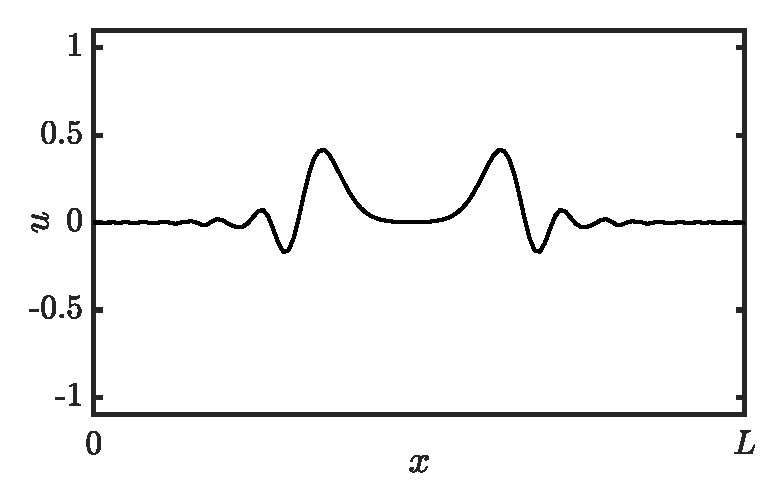
\includegraphics[width=\figWidth\textwidth]{figures/resonators/dispersion2.eps}}\hfill
    \subfloat[$t = 2$ ms.\label{fig:dispersion3}]{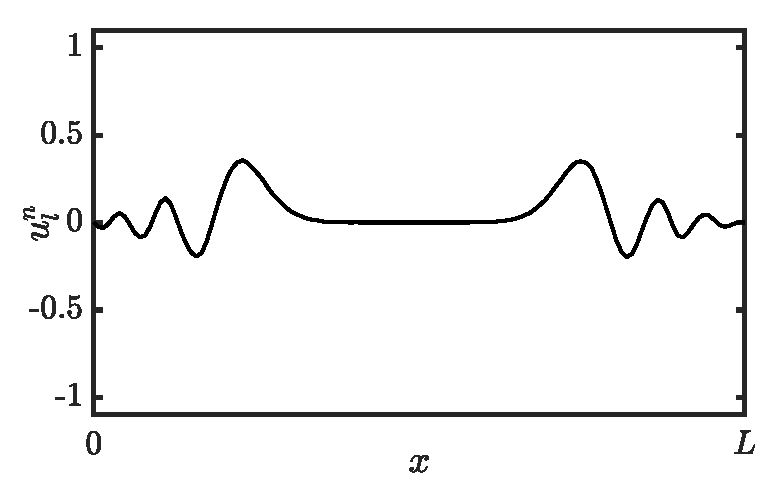
\includegraphics[width=\figWidth\textwidth]{figures/resonators/dispersion3.eps}}
    \caption{Dispersion in a stiff string due to stiffness.\label{fig:dispersion}}
\end{figure}

% \subsubsection{Dispersion Analysis \SWcomment[or: Frequency Dispersion]}
% The 4\thOrder spatial derivative models \textit{frequency dispersion}, a phenomenon that causes different frequencies to travel at different speeds. As opposed to the undesired numerical dispersion 

% \SWcomment[not done]

\subsection{Adding Losses}
Before moving on to the discretisation of the PDE in Eq. \eqref{eq:stiffStringPDENoLosses}, losses can be added to the system. In the physical world, strings lose energy through fx. air viscosity and thermoelastic effects. All frequencies lose energy and die out (damp) over time, but higher frequencies do so at a much faster rate. This phenomenon is called \textit{frequency-dependent damping} and can be modelled using a mixed derivative $\pt \pxx$. This way of frequency-dependent damping first appeared in \cite{Bensa2003} and has been used extensively in the literature since\todo{citations here?}. A damped stiff string can be modelled as
\begin{equation}\label{eq:stiffStringPDE}
    \rho A \ptt u = T \pxx u - EI \pxxxx u - 2 \sz \rho A \pt u + 2 \so \rho A\pt \pxx u,
\end{equation}
where the non-negative loss coefficients $\sz$ (in s$^{-1}$) and $\so$ (in m$^2$/s) determine the frequency-independent and frequency-dependent losses respectively. 

A more compact way to write Eq. \eqref{eq:stiffStringPDE}, and as is also found often in the literature \cite{theBible}\todo{etc.}, is to divide both sides by $\rho A$ to get
\begin{equation}\label{eq:stiffStringPDECompact}
    \ptt u = c^2 \pxx u - \kappa^2 \pxxxx u - 2 \sz \pt u + 2 \so \pt \pxx u
\end{equation}
where $c=\sqrt{T/\rho A}$ is the wave speed \todo{check wavespeed or wave speed (entire document)} (in m/s) as in the 1D wave equation in \eqref{eq:1DwavePDE} and $\kappa = \sqrt{EI / \rho A}$ is referred to as the stiffness coefficient (in m$^2$/s).

% \subsubsection{Intuition}
% Although Eq. \eqref{eq:stiffStringPDE} might look daunting at first, the principle of Newton's second law remains the same. 

% \SWcomment[Something about the 4th spatial derivative and the loss terms here...]

\subsubsection{Boundary Conditions}
Section \ref{sec:1DWave} presents two types of boundary conditions for the 1D wave equation in Eq. \eqref{eq:boundaryCond1DWave}. In the case of the stiff string, these can be extended to
\begin{subequations}\label{eq:stiffStringBoundConds}
    \begin{align}
        u = \px u &= 0 \quad \text{(clamped)}\label{eq:BCclamped}\\
        u = \pxx u &= 0 \quad \text{(simply supported)}\label{eq:BCsimplySupported}\\
        \pxx u = \pxxx u &= 0 \quad \text{(free)}\label{eq:BCfree}
    \end{align}
\end{subequations}
at $x = 0, L$. See Figure \ref{fig:boundaryCondsStiffString} for plots of the first modal shape for each respective boundary condition. 
\def\figWidth{0.32}
\begin{figure}[h]
    \centering
    \subfloat[Clamped.\label{fig:clamped}]{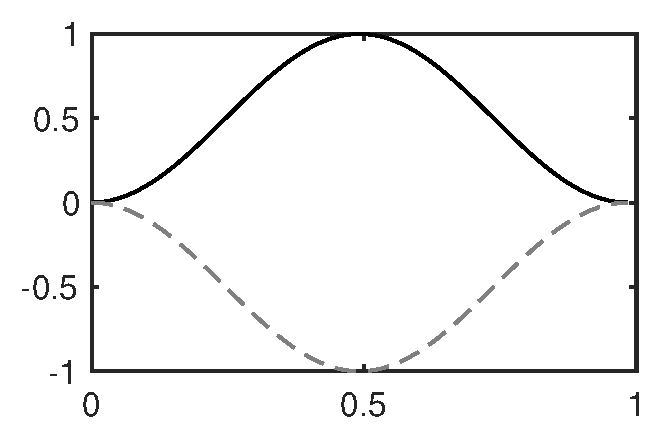
\includegraphics[width=\figWidth\textwidth]{figures/resonators/clamped.eps}}\hfill
    \subfloat[Simply supported.\label{fig:simplySupported}]{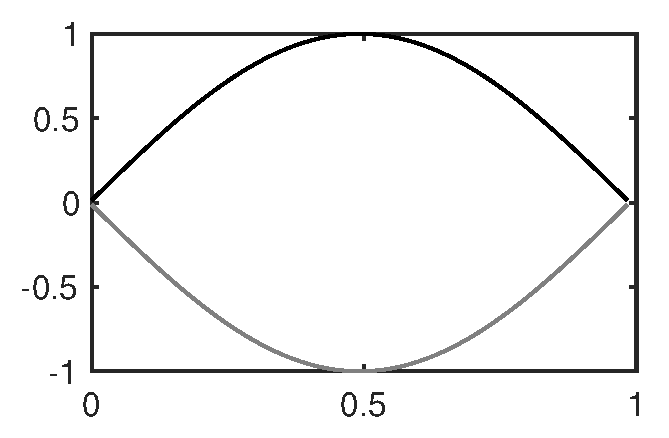
\includegraphics[width=\figWidth\textwidth]{figures/resonators/simplySupported.eps}}\hfill
    \subfloat[Free.\label{fig:free}]{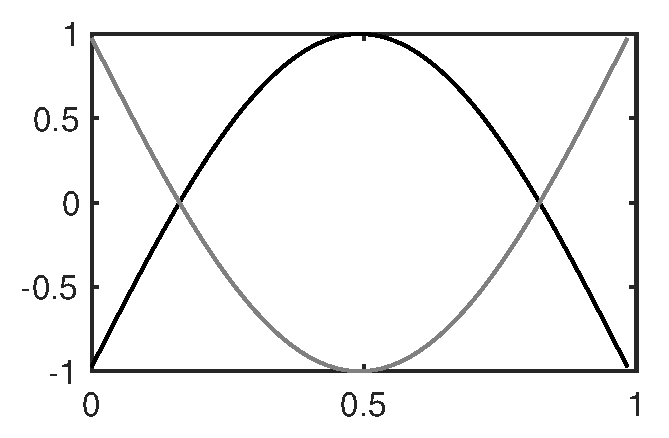
\includegraphics[width=\figWidth\textwidth]{figures/resonators/free.eps}}
    \caption{Plots of the first (normalised) modal shape for the three boundary conditions in Eqs. \eqref{eq:stiffStringBoundConds}. The extremes are indicated with black and grey lines respectively. \label{fig:boundaryCondsStiffString}}
\end{figure}

\section{Discrete Time}\label{sec:stiffStringDiscrete}
For the sake of compactness, we continue with Eq. \eqref{eq:stiffStringPDECompact}, rather than Eq. \eqref{eq:stiffStringPDE}. Naturally, same process can be followed for the latter, the only difference being a multiplication by $\rho A$ of all terms.

Equation \eqref{eq:stiffStringPDECompact} can be discretised as 
\begin{equation}\label{eq:stiffStringFDS}
    \dtt \uln = c^2 \dxx \uln - \kappa^2 \dxxxx \uln - 2 \sz \dtd \uln + 2 \so\dtm\dxx \uln,
\end{equation}
and is defined for domain $l\in\{0, \hdots, N\}$ and number of grid points $N+1$. 
The $\dxxxx$ operator is defined as the second-order spatial difference in Eq. \eqref{eq:discSecondSpace} applied to itself:
\begin{equation}\label{eq:dxxxx}
    \dxxxx = \dxx\dxx = \frac{1}{h^4}\left(e_{x+}^2 - 4e_{x+}+6 - 4e_{x-}+e_{x-}^2\right).
\end{equation} 
A multiplication of two shift operators applied to a grid function simply means to apply each shift individually. The $\dxxxx$ operator applied to $\uln$ thus becomes
\begin{equation}
    \dxxxx\uln = \frac{1}{h^4}\left(u_{l+2}^n - 4u_{l+1}^n+6\uln - 4u_{l-1}^n+u_{l-2}^n\right).
\end{equation}

A definition for the mixed-derivative operator can similarly be found.
Recalling the definitions for $\dtm$ in Eq. \eqref{eq:backwardTimeOperator} and $\dxx$ Eq. \eqref{eq:discSecondSpace}, their combination results in
\begin{align}
    \dtm\dxx &= \frac{1}{k}\left(1-e_{t-}\right)\frac{1}{h^2}\left(e_{x+}-2+e_{x-}\right),\nonumber \\
    &= \frac{1}{kh^2}\left(e_{x+}-2+e_{x-} - e_{t-}(e_{x+}-2+e_{x-})\right).
\end{align}
Two different shift operators multiplied together still simply means to apply each of them to the grid function individually. The $\dtm\dxx$ operator applied to $\uln$ thus yields
\begin{equation}
    \dtm \dxx \uln = \frac{1}{hk^2}\left(u_{l+1}^n - 2 \uln + u_{l-1}^n - u_{l+1}^{n-1} + 2 u_l^{n-1} - u_{l-1}^{n-1}\right).
\end{equation}
The reason a backwards difference is used here is to keep the system \textit{explicit}. A scheme is explicit if the values of $u_l^{n+1}$ can explicitly be calculated from known values. If this is not the case and values of fx. $u_{l+1}^{n+1}$ and $u_{l-1}^{n+1}$ are required to calculate $u_l^{n+1}$, the scheme is called an \textit{implicit}. An example of an implicit scheme using the centred operator for the temporal derivative in the frequency-dependent damping term instead can be found in Section \ref{sec:implicitStiffString}.

With these definitions, 
the operators in scheme \eqref{eq:stiffStringFDS} can be expanded to get
\begin{equation}
    \begin{aligned}\label{eq:expandedStringFDS}
        \frac{1}{k^2}\big(u_l^{n+1} - 2\uln & + u_l^{n-1} \big) =\frac{c^2}{h^2}\left(u_{l+1}^n - 2\uln + u_{l-1}^n\right) \\
        &- \frac{\kappa^2}{h^4}\left(u_{l+2}^n - 4u_{l+1}^n+6\uln - 4u_{l-1}^n+u_{l-2}^n\right) \\ 
        &- \frac{\sz}{k} \left(u_l^{n+1} - u_l^{n-1}\right)\\
        & + \frac{2\so}{kh^2}\left(u_{l+1}^n - 2\uln + u_{l-1}^n - u_{l+1}^{n-1} + 2u_l^{n-1} + u_{l-1}^{n-1}\right),
    \end{aligned}
\end{equation}
and after multiplication by $k^2$ and collecting the terms yields
\begin{equation}
    \begin{aligned}
        (1+\sz k) u_l^{n+1} =&\ \left(2 - 2\lambda^2 - 6\mu^2 - \frac{4\so k}{h^2}\right) \uln\\
        & + \left(\lambda^2 + 4\mu^2 + \frac{2\so k}{h^2}\right) (u_{l+1}^n + u_{l-1}^n) \\
        &- \mu^2 (u_{l+2}^n + u_{l-2}^n) + \left(-1+\sz k + \frac{4\so k}{h^2}\right)u_l^{n-1}\\
        & - \frac{2\so k}{h^2}(u_{l+1}^{n-1} + u_{l-1}^{n-1}),
    \end{aligned}
\end{equation}
with 
\begin{equation}\label{eq:stiffStringCourant}
    \lambda = \frac{ck}{h} \qaq \mu = \frac{\kappa k}{h^2}.
\end{equation}
The update equation follows by dividing both sides by $(1+\sz k)$. 

The stability condition for the FD scheme in \eqref{eq:stiffStringFDS} is defined as 
\begin{equation}\label{eq:stiffStringStability}
    h \geq \sqrt{\frac{c^2k^2+4\so k + \sqrt{(c^2k^2 + 4\so k)^2+16\kappa^2k^2}}{2}},
\end{equation}
and will be derived in Section \ref{sec:stiffStringStability} using von Neumann analysis. 
This condition can then be used to calculate the number of intervals $N$ in a similar fashion as for the 1D wave equation shown in Eq. \eqref{eq:orderOfCalc}. First, Eq. \eqref{eq:stiffStringStability} should be satisfied with equality, after which
\begin{equation*}
    N := \floor[\frac{L}{h}], \qaq h := \frac{L}{N}
\end{equation*}
which can then be used to calculate $\lambda$ and $\mu$ in \eqref{eq:stiffStringCourant}.

\subsubsection{Stencil}
As done in Section \ref{sec:1DWaveDisc}, a stencil for the FD scheme implementing the damped stiff string can be created. This is shown in Figure \ref{fig:stencilStiffString}. In order to calculate $u_l^{n+1}$, $5$ points at the current time step are needed due to the 4\thOrder spatial derivative. Due to the mixed derivative in the frequency-dependent damping term neighbouring points at the previous time step are also required. 
%, the coefficient multiplied onto $u_l^{n+1}$.

% and the terms collected to obtain the following update equation
% \begin{equation}
%     \begin{aligned}
%     % (1+\sz k) u_l^{n+1} =&\ \left(2 - 2\lambda^2 - 6\mu^2 - \frac{4\so k}{h^2}\right) \uln\\
%     % & + \left(\lambda^2 + 4\mu^2 + \frac{2\so k}{h^2}\right) (u_{l+1}^n + u_{l-1}^n) \\
%     % &- \mu^2 (u_{l+2}^n + u_{l-2}^n) + \left(-1+\sz k + \frac{4\sz k}{h^2}\right)u_l^{n-1}\\
%     % & - \frac{2\so k}{h^2}(u_{l+1}^{n-1} + u_{l-1}^{n-1})
%     % \end{aligned}
%     Au_l^{n+1} = &\ B_0 \uln + B_1 (u_{l+1}^n + u_{l-1}^n) + B_2 (u_{l+2}^n + u_{l-2}^n) \\
%     &+ C_0 u_l^{n-1} + C_1(u_{l+1}^{n-1} + u_{l-1}^{n-1}) 
%     \end{aligned}
% \end{equation}
% with coefficients
% \begin{gather*}
%     B_0 = 2 - 2\lambda^2 - 6\mu^2 - \frac{4\so k}{h^2}, \quad B_1 = \lambda^2 + 4\mu^2 + \frac{2\so k}{h^2}, \quad B_2 =- \mu^2, \\[1em]
%     C_0 =  -1+\sz k + \frac{4\so k}{h^2},\quad C_1 = - \frac{2\so k}{h^2}, \qaq A = 1+\sz k.
% \end{gather*}
% Note that for clarity the division by $A$ has been left for implementation. 
\begin{figure}[h]
    \centering
    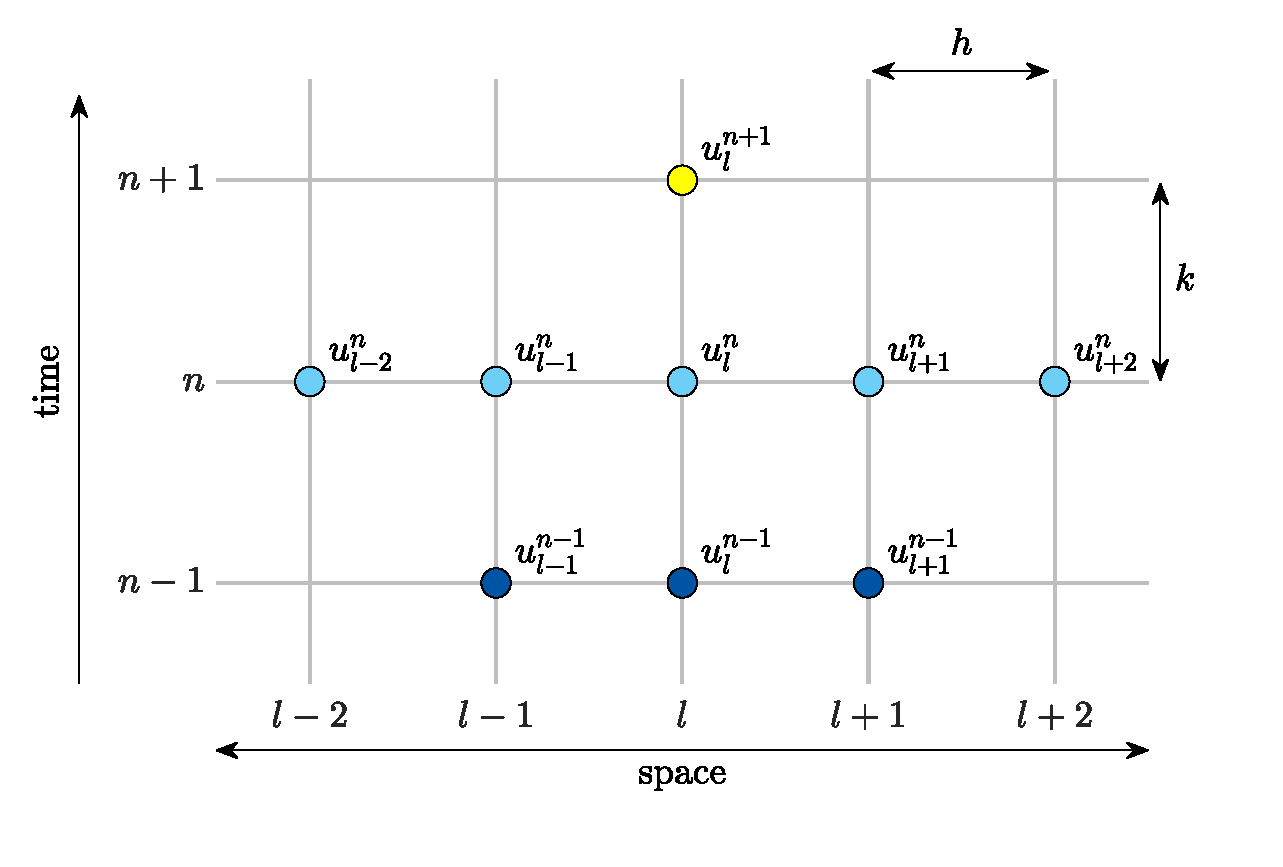
\includegraphics[width=0.8\textwidth]{figures/resonators/stencilDampedStiffString.eps}
    \caption{The stencil for the damped stiff string scheme in Eq. \eqref{eq:stiffStringFDS}. (Adapted from \citeP[A].)\label{fig:stencilStiffString}}
\end{figure}

\subsection{Boundary conditions}\label{sec:stiffStringBoundaryConditions}
Due to the 4\thOrder spatial derivative, two virtual grid points need to be accounted for at the boundaries of the system. Discretising the boundary conditions in \eqref{eq:stiffStringBoundConds} yields
\begin{subequations}\label{eq:stiffStringBoundCondsDisc}
    \begin{align}
        \uln = \delta_{x\pm} \uln &= 0 \quad \text{(clamped)}\label{eq:BCclampedDisc}\\
        \uln = \dxx \uln &= 0 \quad \text{(simply supported)}\label{eq:BCsimplySupportedDisc}\\
        \dxx \uln = \dxd\dxx \uln &= 0 \quad \text{(free)}\label{eq:BCfreeDisc}
    \end{align}
\end{subequations}
at $l = 0, N$. The operator in the clamped condition uses the $\dxp$ operator at the left boundary ($l = 0$) and $\dxm$ at the right ($l = N$). Note that for the free boundary condition in Eq. \eqref{eq:BCfree}, to discretise $\px^3$ the more accurate $\dxd\dxx$ operator has been chosen over the less accurate $\dxm \dxx$ and $\dxp \dxx$ operators for the left and right boundary respectively.

Below, the boundary conditions are expanded to get definitions for the virtual grid points. 

\todo{insert figure showing virtual grid points somewhere in this section}

\subsubsection{Clamped}
Expanding the operators for the clamped condition yields 
\begin{equation}
    u_0^n = u_1^n = 0 \qaq u_{N-1}^n = u_N^n = 0.
\end{equation}
This can be simplified by reducing the range of calculation to $l\in \{ 2, \hdots, N-2\}$.

\subsubsection{Simply supported}
As the states of the end points of a system with simply supported boundary conditions are $0$ at all times, the range of calculation can be reduced to $l\in \{ 1, \hdots, N-1\}$. At $l=1$ and $l=N-1$, definitions for the virtual grid points $u_{-1}^n$ and $u_{N+1}^n$ are needed. A definition for $u_{-1}^n$ can be found by expanding Eq. \eqref{eq:BCsimplySupportedDisc} at $l = 0$:
\begin{align}
    &\frac{1}{h^2}\left(u_1^n - 2 u_0^n + u_{-1}^n\right) = 0,\nonumber\\[-1em]
    \xLeftrightarrow{\mystrut\ u^n_0 = 0\ } \quad & u_1^n + u_{-1}^n = 0,\nonumber\\[0.25em]
    &u_{-1}^n = -u_1^n,\label{eq:simplySupportedResult}
\end{align}
and similarly for $u_{N+1}^n$ by expanding the condition at $l=N$:
\begin{equation*}
    u_{N+1}^n = -u_{N-1}^n.
\end{equation*}
Filling the first definition into the expanded scheme at $l=1$ in \eqref{eq:expandedStringFDS} and collecting the terms yields
\begin{equation}
    \begin{aligned}
        \!\!\!\!\!(1+\sz k) u_1^{n+1} =&\ \left(2 - 2\lambda^2 - 5\mu^2 - \frac{4\so k}{h^2}\right) u_1^n + \left(\lambda^2 + 4\mu^2 + \frac{2\so k}{h^2}\right) u_{2}^n \\
        &-\mu^2u_3^n+ \left(-1+\sz k + \frac{4\sz k}{h^2}\right)u_1^{n-1} - \frac{2\so k}{h^2}u_{2}^{n-1}.
    \end{aligned}
\end{equation}
Doing the same for $l=N-1$, we get
\begin{equation}
    \begin{aligned}
        \!\!\!\!\!(1+\sz k) u_{N-1}^{n+1} =&\ \left(2 - 2\lambda^2 - 5\mu^2 - \frac{4\so k}{h^2}\right) u_{N-1}^n + \left(\lambda^2 + 4\mu^2 + \frac{2\so k}{h^2}\right) u_{N-2}^n \\
        &-\mu^2u_{N-3}^n+ \left(-1+\sz k + \frac{4\sz k}{h^2}\right)u_{N-1}^{n-1} - \frac{2\so k}{h^2}u_{N-2}^{n-1}.
    \end{aligned}
\end{equation}

\subsubsection{Free}
Finally, the free boundary condition requires all points to be calculated and the range of calculation is $l\in\{0, \hdots, N\}$. At each respective boundary, two virtual grid points are needed: $u_{-1}^n$ and $u_{-2}^n$ at the left and $u_{N+1}^n$ and $u_{N+2}^n$ at the right boundary respectively.
The combined operator in Eq. \eqref{eq:BCfreeDisc} is defined as:
\begin{align}
    \dxd\dxx &= \frac{1}{2h^3}\left(e_{x+}-e_{x-}\right)\left(e_{x+}-2+e_{x-}\right),\nonumber\\
    &=\frac{1}{2h^3}\left(e_{x+}^2 - 2e_{x+} + 1 - (1 - 2e_{x-} + e_{x-}^2\right),\nonumber\\
    &=\frac{1}{2h^3}\left(e_{x+}^2 - 2e_{x+} + 2e_{x-} -e_{x-}^2\right),
\end{align}
and can be used to solve for $u_{-2}^n$ at $l=0$:
\begin{align*}
    \frac{1}{2h^3} &\left(u_2^n - 2 u_1^n + 2u_{-1}^n - u_{-2}^n\right) = 0,\\%[0.25em]
    u_{-2}^n &= u_2^n - 2 u_1^n + 2u_{-1}^n.
    % \\[-1em]
    % \!\!\!\!\!\!\!\!\!\!\!\!\!\!\!\xLeftrightarrow{\mystrut\ \dxx \uln = 0\ \Rightarrow\ \text{ Eq. \eqref{eq:simplySupportedResult}}\ }
    % \quad u_{-2}^n &= u_2^n - 4 u_1^n 
\end{align*}
As $u_0^n$ is not necessarily $0$ at all times, solving the first part of the boundary condition yields a different result than in the simply supported case:
\begin{align*}
    \frac{1}{h^2} &\left(u_1^n - 2 u_0^n + u_{-1}^n \right) = 0,\\
    u_{-1}^n &= 2u_0^n - u_1^n.
    % \\[-1em]
    % \!\!\!\!\!\!\!\!\!\!\!\!\!\!\!\xLeftrightarrow{\mystrut\ \dxx \uln = 0\ \Rightarrow\ \text{ Eq. \eqref{eq:simplySupportedResult}}\ }
    % \quad u_{-2}^n &= u_2^n - 4 u_1^n 
\end{align*}
The same can be done at $l=N$ to get the following definitions for the virtual grid points
\begin{equation*}
    u_{N+2}^n = u_{N-2}^n - 2 u_{N-1}^n + 2u_{N+1}^n
    \qaq u_{N+1}^n = 2u_N^n - u_{N-1}^n.
\end{equation*}
The update equations for the boundary points will not be given here. Instead the matrix form of the FD scheme with free boundaries will be provided below. 
% The update equation at $l=0$ then becomes
% \begin{equation}
%     \begin{aligned}
%         \!\!\!\!\!(1+\sz k) u_0^{n+1} =&\ \left(2 - 2\lambda^2 - 2 \mu^2 - \frac{4\so k}{h^2}\right) u_0^n + \left(\lambda^2 +4\mu^2 + \frac{4\so k}{h^2}\right) u_1^n \\
%         &-2\mu^2u_2^n+ \left(-1+\sz k + \frac{4\sz k}{h^2}\right)u_0^{n-1} - \frac{4\so k}{h^2}u_1^{n-1}.
%     \end{aligned}
% \end{equation}
% at $l=1$
% \begin{equation}
%     \begin{aligned}
%         \!\!\!\!\!(1+\sz k) u_1^{n+1} =&\ \left(2 - 2\lambda^2 - 5\mu^2 - \frac{4\so k}{h^2}\right) u_1^n + \left(\lambda^2 + 4\mu^2 + \frac{2\so k}{h^2}\right) u_{2}^n \\
%         &-2\mu^2u_3^n+ \left(-1+\sz k + \frac{4\sz k}{h^2}\right)u_1^{n-1} - \frac{2\so k}{h^2}u_{2}^{n-1}.
%     \end{aligned}
% \end{equation}

In practice, the simply supported boundary condition is mostly chosen as this reflects reality the most. The clamped condition could be chosen for simplicity as this does not require an alternative update at the boundaries. The free boundary condition is more often used to model a (damped) ideal bar, (Eq. \eqref{eq:stiffStringPDE} with $T = 0$).

\subsection{Implementation and Matrix Form}\label{sec:implementationStiffString}
When using \texttt{MATLAB}, for a more compact implementation, it is useful to write the scheme in matrix form. The FD scheme of the stiff string in \eqref{eq:stiffStringFDS} can be written as 
\begin{equation}\label{eq:matrixFormStiffString}
    A\u^{n+1} = \B\u^n + \C \u^{n-1}
\end{equation}
where 
\begin{equation*}
    \begin{gathered}
    A = (1+\sz k), \quad \B = 2\I + c^2 k^2 \Dxx - \kappa^2 k^2 \Dxxxx + 2 \so k \Dxx, \\
    \text{and} \quad \C = -(1-\sz k)\I - 2\so k \Dxx.
    \end{gathered}
\end{equation*}
Notice that $A$ is a scalar rather than a matrix.

The size of the state vectors and the matrix-form operators depend on the boundary conditions. For clamped conditions, the state vectors ($\u^{n+1}$, $\u^n$ and $\u^{n-1}$) and matrices will be of size $(N-3) \times 1$ and $(N-3) \times (N-3)$ respectively. The $\Dxx$ matrix will be of the form given in \eqref{eq:DxxDef} and the matrix form of the $\dxxxx$ operator is
\begin{equation}
    \mathbf{D}_{xxxx} = \frac{1}{h^4}\begin{bmatrix}
        6& -4 & 1 & & \mathbf{0} \\
        -4 & 6 &\ddots &\ddots & \\
        1& \ddots & \ddots & \ddots&1 \\
        &\ddots & \ddots & 6 & -4 \\
        \mathbf{0} & & 1& -4 & 6 \\
    \end{bmatrix}.
\end{equation}

For simply supported conditions, the state vectors and matrices will be of size $(N-1) \times 1$ and $(N-1) \times (N-1)$ respectively. Again, $\Dxx$ is as defined in \eqref{eq:DxxDef} and $\Dxxxx$ can be obtained by multiplying two $\Dxx$ matrices according to 
\begin{equation}
    \mathbf{D}_{xxxx} = \Dxx\Dxx = \frac{1}{h^4}\begin{bmatrix}
        5& -4 & 1 & & & \mathbf{0}& \\
        -4 & 6 &\ddots &\ddots & & & \\
        1& \ddots & \ddots & -4 & 1 & & \\
        & \ddots& -4 & 6 & -4 & \ddots& \\
        & & 1 & -4 & \ddots & \ddots &1 \\
        & & & \ddots & \ddots & 6 & -4 \\
        & \mathbf{0} & & & 1& -4 & 5 \\
    \end{bmatrix}.
\end{equation}

Finally for free boundary conditions as given in \eqref{eq:BCfreeDisc}, the state vectors and matrices are $(N+1)\times 1$ and $(N+1)\times (N+1)$ respectively. Now, the $\Dxx$ matrix is of the form in \eqref{eq:DxxDefNeumann} instead, and

\setstackgap{L}{16pt}
\setstacktabbedgap{8pt}
\def\lrgap{\kern3pt}
\fixTABwidth{T}
\begin{equation}
    \mathbf{D}_{xxxx} = \frac{1}{h^4}\xbracketMatrixstack{
        2& -4 & 2 & & & \mathbf{0}& \\
        -2 & 5 & -4 & 1 & & & \\
        1& -4 & 6 & -4 & 1 & & \\
        & \ddots & \ddots & \ddots & \ddots &\ddots & \\
        & & 1 & -4 & 6 & -4 &1 \\
        & & & 1 & -4 & 5 & -2 \\
        & \mathbf{0} & & & 2& -4 & 2}.
\end{equation}

\subsection{Parameters and output}\label{sec:paramsAndOutput}
The values of the parameters naturally determine the properties of the output sound. Where in the 1D wave equation, only the fundamental frequency $f_0$ could be affected, the stiff string has much more aspects that can be changed. See Table \ref{tab:stiffStringParams} for parameters most commonly used in this project. There exists a formula to calculate the loss coefficients $\sz$ and $\so$ from $T_{60}$ values at different frequencies (see \cite[Eq (7.29)]{theBible}). During this project, however, these values have been tuned by ear and are usually set to be approximately those found in Table \ref{tab:stiffStringParams}. 

\begin{table}[h]
    \begin{center}
    \begin{tabular}{|l|c|c|}
        \hline
        Name & Symbol (unit) & Value\\ \hline
        Length & $L$ (m) & $1$\\
        Material density & $\rho$ (kg/m$^3$) & $7850$\\
        Radius & $r$ (m) & $5\cdot10^{-4}$\\
        Tension & $T$ (N) &$100 \leq T \leq 1.5\cdot 10^4$\\
        Young's modulus & $E$ (Pa) & $2\cdot10^{11}$\\
        Freq.-independent damping & $\sz$ (s$^{-1}$) & $1$\\
        Freq.-dependent damping & $\so$ (m$^2$/s) & $0.005$\\\hline
    \end{tabular}
    \caption{Parameters and their values most commonly used over the course of this project.\label{tab:stiffStringParams}}
    \end{center}
\end{table}
{\renewcommand{\arraystretch}{1}


\subsubsection{Output}
Figure \ref{fig:stiffStringOutput} shows the time-domain and frequency-domain output (retrieved at $l = 3$) of an implementation of the stiff string excited using a raised-cosine. The parameters used can be found in Table \ref{tab:stiffStringParams} 
with $T = 1129$. Furthermore, $E = 7\cdot 10^{11}$ to highlight dispersive effects. Finally, simply supported boundary conditions are chosen. From the left panel, one can observe that over time, dispersive effects show where higher-frequency components in the excitation travel faster through the medium than lower-frequency components. In the frequency domain (the right panel in Figure \ref{fig:stiffStringOutput}) this shows in the partials not being perfect integer multiples of the fundamental. Notice that the partials are closer to each other for lower frequencies and further apart as their frequency increases. Finally, the frequency-dependent damping term causes higher frequencies to have a lower amplitude than lower frequencies. 

Apart from the obvious material properties such as density, stiffness and geometry, perceptual qualities of the sound are surprisingly much determined by $\so$, and for lower values the output can become extremely metallic.

\begin{figure}[h]
    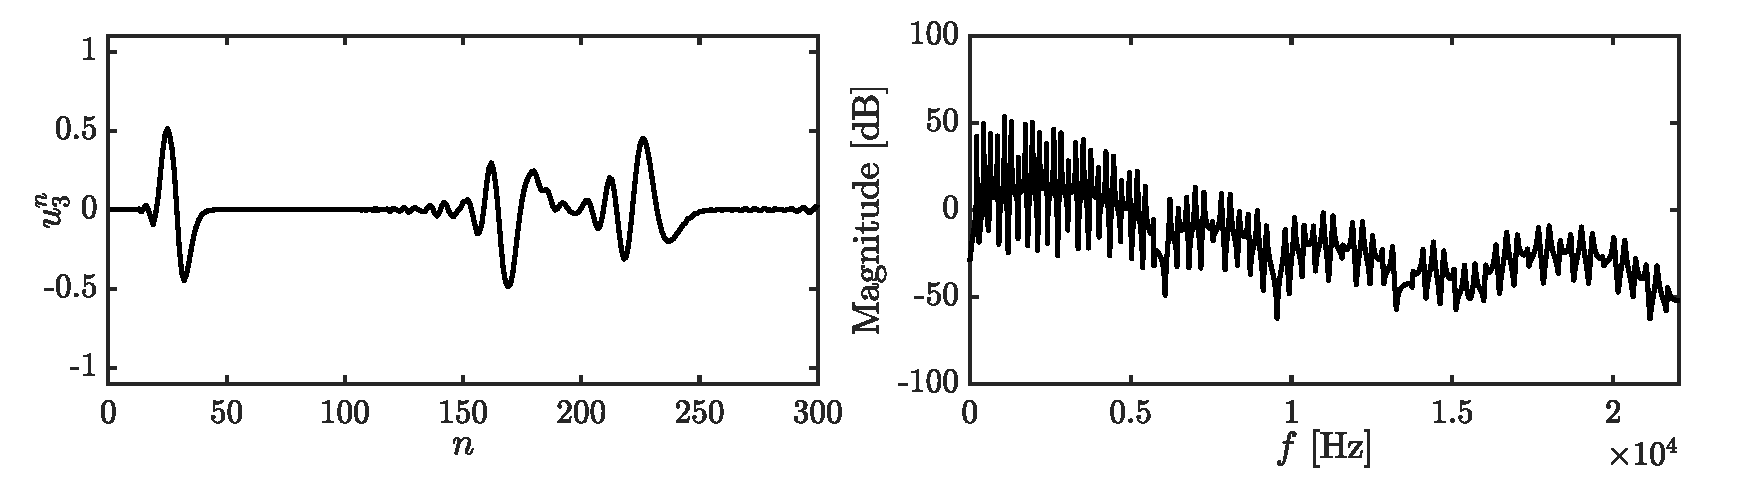
\includegraphics[width=\textwidth]{figures/resonators/outputFFT.eps}
    \caption{The time-domain and frequency-domain output of the stiff string. The parameters are set as in Table \ref{tab:stiffStringParams} with $E = 7\cdot 10^{11}$ to highlight dispersive effects and $T = 1129$. From the left panel, one can observe that over time, dispersive effects show due to the stiffness in the string. In frequency domain (right panel) this shows through the partials not being perfect integer multiples of the fundamental. Lastly, higher frequency components have a lower amplitude due to the frequency-dependent damping.\label{fig:stiffStringOutput}}
\end{figure}


\section{von Neumann Analysis and Stability Condition}\label{sec:stiffStringStability}
In order to obtain the stability condition for the damped stiff string, one can perform von Neumann analysis as presented in Section \ref{sec:stabilityAnalysis} on the FD scheme in Eq. \eqref{eq:stiffStringFDS}.

Using the definitions found in Eq. \eqref{eq:temporalAnsatz} for the temporal operators and Eqs. \eqref{eq:dxxAnsatz} and \eqref{eq:dxxxxAnsatz} for the spatial operators, the frequency-domain representation of Eq. \eqref{eq:stiffStringFDS} can be obtained:
\begin{align*}
    \!\!\!\!\frac{1}{k^2}\left(z - 2 + z^{-1}\right) =&-\frac{4c^2}{h^2}\sin^2(\beta h/2) - \frac{16\kappa^2}{h^4}\sin^4(\beta h/2) - \frac{\sz}{k}z + \frac{\sz}{k}z^{-1}\\
    & - \frac{8 \so}{kh^2}\sin^2(\beta h/2) + \frac{8 \so}{kh^2} \sin^2(\beta h/2)z^{-1},
\end{align*}
and after collecting the terms, the characteristic equation follows:
\begin{gather}
    (1+\sz k)z + \left(16\mu^2\sin^4(\beta h/2)+\left(4\lambda^2+\frac{8\so k}{h^2}\right)\sin^2(\beta h/2) - 2\right)\nonumber\\
    +\left(1-\sz k-\frac{8\so k}{h^2}\sin^2(\beta h/2)\right)z^{-1}=0.\label{eq:charDampedString}
\end{gather}
Rewriting this to the form in Eq. \eqref{eq:polynomialForm}, and using $\S = \sin^2(\beta h /2)$ for brevity, yields
\begin{equation*}
    z^2 + \left(\frac{16\mu^2\S^2+\left(4\lambda^2+\frac{8\so k}{h^2}\right)\S - 2}{1 + \sz k}\right)z+\frac{1-\sz k-\frac{8\so k}{h^2}\S}{1 + \sz k}=0.
\end{equation*}
Stability of the system can then be proven using condition \eqref{eq:condition214} and substituting the coefficients into this condition yields
\begin{equation}\nonumber
    \begin{aligned}
        \left|\frac{16\mu^2\S^2+\left(4\lambda^2+\frac{8\so k}{h^2}\right)\S - 2}{1+\sz k}\right|-1 &\leq \frac{1-\sz k-\frac{8\so k}{h^2}\S}{1+\sz k}\leq 1,\\
        \left|16\mu^2\S^2+\left(4\lambda^2+\frac{8\so k}{h^2}\right)\S - 2\right|-(1+\sz k) &\leq 1-\sz k-\frac{8\so k}{h^2}\S\leq 1+\sz k,\\
        \left|16\mu^2\S^2+\left(4\lambda^2+\frac{8\so k}{h^2}\right)\S - 2\right|&\leq2-\frac{8\so k}{h^2}\S\leq2+2\sz k.
    \end{aligned}
\end{equation}
The second condition is always true due to the fact that $\sigma_0,\sigma_1 \geq 0$. Continuing with the first condition: 
\begin{align*}
    -2+\frac{8\so k}{h^2}\S&\leq 16\mu^2\S^2+\left(4\lambda^2+\frac{8\so k}{h^2}\right)\S - 2\leq 2-\frac{8\so k}{h^2}\S,\\
    0&\leq 16\mu^2\S^2+4\lambda^2\S\leq 4-\frac{16\so k}{h^2}\S.
\end{align*}
As $16\mu^2\S^2+4\lambda^2\S$ is non-negative, the first condition is always satisfied. Continuing with the second condition:
\begin{align*}
    16\mu^2\S^2+\left(4\lambda^2+ \frac{16\so k}{h^2}\right)\S &\leq 4,\\
    4\mu^2\S^2+\left(\lambda^2+ \frac{4\so k}{h^2}\right)\S&\leq 1.
\end{align*}
As $\S$ is bounded by $1$, this can be substituted as it challenges the condition the most. \todo{different wording} Continuing with the substituted definitions for $\lambda$ and $\mu$ from Eq. \eqref{eq:stiffStringCourant} yields
\begin{align*}
    \frac{4\kappa^2k^2}{h^4}+\frac{c^2k^2 + 4\so k}{h^2}&\leq 1, \\
    4\kappa^2k^2+(c^2k^2+ 4\so k)h^2&\leq h^4,\\
    h^4- (c^2k^2+ 4\so k)h^2 - 4\kappa^2k^2 &\geq 0 ,
\end{align*}
which is a quadratic equation in $h^2$. Using the quadratic formula, the grid spacing $h$ can then be shown to be bounded by
\begin{equation}
    h \geq \sqrt{\frac{c^2k^2+4\so k + \sqrt{(c^2k^2 + 4\so k)^2+16\kappa^2k^2}}{2}},
\end{equation}
which is the stability condition for the damped stiff string also shown in Eq. \eqref{eq:stiffStringStability}.

\section{Energy Analysis}\label{sec:energyAnalysisString}
As mentioned in Section \ref{sec:energyAnalysis}, it is useful to perform the energy analysis on the scheme with all physical parameters written out. Discretising the PDE in \eqref{eq:stiffStringPDE} yields
\begin{equation}
    \rho A \dtt \uln = T \dxx \uln - EI \dxxxx \uln - 2\sz \rho A \dtd \uln + 2 \so \rho A \dtm \dxx \uln,
\end{equation}
defined for $l\in d$ with discrete domain $d = \{0, \hdots, N\}$. This section will follow the 4 steps described in Section \ref{sec:energyAnalysis}.

\subsubsection{Step 1: Obtain $\dtp \h$}
The first step is to take the inner product (see Eq. \eqref{eq:discInnerProd}) of the scheme with $(\dtd \uln)$ over discrete domain $d$:
\begin{equation}\label{eq:rOCStiffString}
    \begin{aligned}
    \dtp \h =&\ \rho A \langle \dtd \uln, \dtt \uln \rangle_d - T \langle \dtd \uln, \dxx \uln\rangle_d + EI \langle \dtd \uln, \dxxxx \uln \rangle_d\\
    & + 2\sz\rho A \langle \dtd \uln, \dtd \uln \rangle_d - 2\so \rho A\langle \dtd \uln, \dtm \dxx \uln \rangle_d = 0.
    \end{aligned}
\end{equation}  
% If the free boundary conditions in \eqref{eq:BCfreeDisc} are used, the primed inner product in Eq. \eqref{eq:primedInnerProd} needs to be used. Here we continue with clamped / simply supported boundaries.

\subsubsection{Step 2: Identify energy types and isolate $\dtp$}
As there is damping present in the system, and the system is distributed, the damping term $\mathfrak{q}$ and boundary term $\mathfrak{b}$ appear and the energy balance will be of the form 
\begin{equation}
    \dtp \h = \mathfrak{b}-\mathfrak{q}.
\end{equation}
The damping term is defined as \todo{virtual grid points needed for freq-dep damping term..}
\begin{equation}\label{eq:dampingTermStiffString}
    \mathfrak{q} = 2\sz \rho A \lVert\dtd\uln\rVert_d^2 - 2 \so \rho A \langle \dtd \uln, \dtm \dxx \uln \rangle_d,
\end{equation}
and the boundary term $\mathfrak{b}$ appears after rewriting Equation \eqref{eq:rOCStiffString} using summation by parts (see Section \ref{sec:summationByParts}). Specifically, using Eq. \eqref{eq:summationByPartsMinusBar} for the second term and Eq. \eqref{eq:summationByPartsTwiceReduced} for the third, we get
\begin{align*}
    \dtp \h &= \rho A \langle \dtd \uln, \dtt \uln \rangle_d + T \langle \dtd \dxp \uln, \dxp \uln\rangle_{\underline{d}} + EI \langle \dtd \dxx \uln, \dxx \uln \rangle_{\overline{\underline{d}}} \\
    &= \mathfrak{b} - \mathfrak{q}
\end{align*}
where the boundary term becomes
\begin{align*}
    \mathfrak{b} =&\ T\Big((\dtd u_N^n)(\dxp u_N^n) - (\dtd u_0^n) (\dxp u_{-1}^n)\Big) \\
    &+ EI \Big((\dtd u_N^n)(\dxp \dxx u_N^n) - (\dxx u_N^n)(\dxm \dtd u_N^n) \Big)\\
    &+ EI \Big(- (\dtd u_0^n)(\dxm \dxx u_0^n) + (\dxx u_0^n)(\dxp \dtd u_0^n)\Big).
\end{align*}
For the clamped and simply supported boundary conditions in \eqref{eq:BCclampedDisc} and \eqref{eq:BCsimplySupportedDisc} it can easily be shown that $\mathfrak{b} = 0$. If free conditions as in Eq. \eqref{eq:BCfreeDisc} are used, the boundary conditions will vanish when the primed inner product in Eq. \eqref{eq:primedInnerProd} is used in Step 1 and identity \eqref{eq:summationByPartsTwicePrimed} is used when performing summation by parts. Here, we continue with the clamped / simply supported case. 

Isolating $\dtp$ to obtain the total energy $\h$ in the definition for $\dtp \h$ above, requires identities \eqref{eq:prodIdentity1} and \eqref{eq:prodIdentity2} and yields
\begin{equation*}
    \begin{aligned}
        \dtp\h &= \dtp\left(\frac{\rho A}{2}\lVert\dtm \uln\rVert_d^2 + \frac{T}{2}\langle\dxp\uln, e_{t-}\dxp\uln\rangle_{\underline{d}} + \frac{EI}{2}\langle\dxx\uln, e_{t-}\dxx\uln\rangle_{\overline{\underline{d}}}\right) \\
        &=-\mathfrak{q}.
    \end{aligned}
\end{equation*}
From this, the definition for the Hamiltonian $\h$, the kinetic energy $\t$ and potential energy $\v$ can be found:
\begin{equation}\label{eq:energyBalanceStiffString}
    \begin{gathered}
        \h = \t + \v, \qwiq \t = \frac{\rho A}{2}\lVert\dtm \uln\rVert^2_d,\quad \text{and} \\
        \v = \frac{T}{2}\langle\dxp\uln, e_{t-}\dxp\uln\rangle_{\underline{d}} + \frac{EI}{2}\langle\dxx\uln, e_{t-}\dxx\uln\rangle_{\overline{\underline{d}}}\ .
    \end{gathered}
\end{equation}

\subsubsection{Step 3: Check units}
Comparing the acquired energy balance in Eq. \eqref{eq:energyBalanceStiffString} to the energy balance for the 1D wave equation in Eq. \eqref{eq:energyBalance1DWave}, one can observe that the balances are nearly identical, the only difference being the second term in the definition for $\v$ in Eq. \eqref{eq:energyBalanceStiffString}. 
Writing this term out in units, and recalling that Pa (the unit for $E$) in SI units is kg$\cdot$m$^{-1}\cdot$s$^{-2}$, yields
\begin{align*}
    \frac{EI}{2}\langle\dxx\uln, e_{t-}\dxx\uln\rangle_{\overline{\underline{d}}}\overset{\text{in units}}{\xrightarrow{\hspace*{1cm}}}& \ \text{Pa}\cdot \text{m}^4 \cdot \text{m} \cdot (\text{m}^{-2} \cdot \text{m} \cdot \text{m}^{-2} \cdot \text{m}) \\
    & = \text{kg} \cdot \text{m}^2 \cdot \text{s}^{-2},
\end{align*}
and indeed has the correct units. 

The damping terms in $\mathfrak{q}$ need to be in Joules per second, or kg $\cdot$ m$^2 \cdot$ s$^{-3}$. Writing the terms in Eq. \eqref{eq:dampingTermStiffString} out in their units yields
\begin{align*}
    2\sz \rho A \lVert\dtd\uln\rVert_d^2\overset{\text{in units}}{\xrightarrow{\hspace*{1cm}}}&\ \text{s}^{-1}\cdot\text{kg}\cdot\text{m}^{-3}\cdot\text{m}^2\cdot \text{m}\cdot(\text{s}^{-1}\cdot\text{m})^2 \\
    &= \text{kg} \cdot \text{m}^2 \cdot \text{s}^{-3},\\
    - 2 \so \rho A \langle \dtd \uln, \dtm \dxx \uln \rangle_d \overset{\text{in units}}{\xrightarrow{\hspace*{1cm}}}&\  \text{m}^2\cdot\text{s}^{-1}\cdot\text{kg}\cdot\text{m}^{-3}\cdot\text{m}^2\\
    &\cdot\text{m}\cdot(\text{s}^{-1}\cdot\text{m})(\text{s}^{-1}\cdot\text{m}^{-2}\cdot \text{m}),\\
    &= \text{kg} \cdot \text{m}^2 \cdot \text{s}^{-3},
\end{align*}
and also have the correct units.
\subsubsection{Step 4: Implementation}
An implementation of the energy calculation for the simply supported boundary condition is given in Algorithm \ref{alg:stiffStringEnergy}. The damping is ignored but can be found in Appendix \ref{app:stiffstring}. \todo{Add to appendix or refer to a gist} Figure \ref{fig:energyStiffString} shows that the deviation of the total energy calculated using Eq. \eqref{eq:normalisedEnergyDamping} is within machine precision.

\setlstMAT
\begin{lstlisting}[caption=Calculating $\h$ for the simply supported boundary condition., label=alg:stiffStringEnergy]
%%%% Before the main loop: %%%%

% Initialise Dx+ operator to calculate potential energy due to tension
% As the domain is reduced by one, the matrix needs to be of size N x N
Dxp = sparse(1:N, 1:N, -ones(1, N), N, N) + ...
        sparse(1:N-1, 2:N, ones(1, N-1), N, N);

%%%% In the main loop: %%%%

% energy in the system
kinEnergy(n) = rho * A * h / 2 * sum((1/k * (u - uPrev)).^2);
potEnergy(n) = T / 2 * h * sum((Dxp * [0; u]) .* (Dxp * [0; uPrev])) ... + E * I * h / 2 * sum((Dxx * u) .* (Dxx * uPrev));
\end{lstlisting}

\begin{figure}[h]
    \centering
    \begin{tikzpicture}[->,node distance=3cm,
        thick,main node/.style={circle,draw}]
    
        \node[] (image) at (0,0) {
        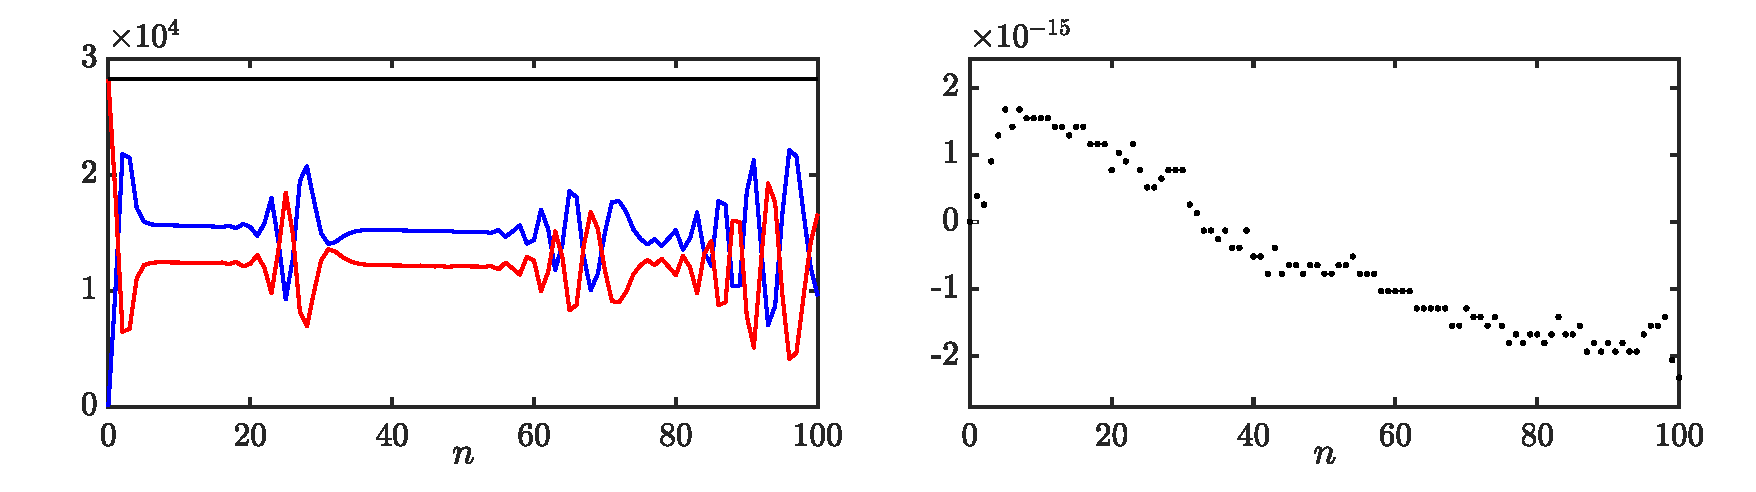
\includegraphics[width=\textwidth]{figures/resonators/stiffStringEnergy.eps}
        };
    
        \node[] (he) at (0.2,0.5) {\small $\mathfrak{h}_\text{e}$};

        \node[] (h) at (-5.75, 1) {\small $\mathfrak{h}$};
        \node[] (v) at (-5.75, 0.5) {\small $\color{red}\mathfrak{v}$};
        \node[] (t) at (-5.75, 0) {\small $\color{blue}\mathfrak{t}$};
      \end{tikzpicture}
      \caption{The kinetic (blue), potential (red), and total (black) energy of an implementation of the stiff string are plotted in the left panel. Notice that the damping present in the system causes $\h$ to decrease. The right panel shows the normalised energy (according to Eq. \eqref{eq:normalisedEnergyDamping}) and shows that the deviation of the energy is within machine precision. \label{fig:energyStiffString}}
\end{figure}

\section{Modal Analysis}
% To find an expression for the modal frequencies one can ignore the damping terms for now and follow the process in Section \ref{sec:modalAnalysis} to obtain
% \begin{equation}
%     f_p = \frac{1}{\pi k}\sin^{-1}\left(\frac{1}{2}\sqrt{-\eig_p(c^2k^2\Dxx - \kappa^2k^2\Dxxxx)}\right).
% \end{equation}

To be able to perform a modal analysis on the FD scheme in \eqref{eq:stiffStringFDS}, it must be written in one-step form -- introduced in Section \ref{sec:oneStepForm} -- due to the damping. Using the matrix form of the damped stiff string in Eq. \eqref{eq:matrixFormStiffString}, the one-step form can be written as
%needs be used. As there are damping terms present in the system, it is useful to write the update in one-step form as explained in Section \ref{sec:oneStepForm}.
\begin{equation}\label{eq:oneStepFormStiffSTring}
    \underbrace{\begin{bmatrix}
        \u^{n+1}\\
        \u^n
    \end{bmatrix}}_{\w^{n+1}} = 
    \underbrace{\begin{bmatrix}
        \B/A & \C/A\\
        \I & \mathbf{0}
    \end{bmatrix}}_{\Q}
    \underbrace{\begin{bmatrix}
        \u^n\\
        \u^{n-1}
    \end{bmatrix}}_{\w^n}
\end{equation}
where the definitions for $\B$, $\C$ and $A$ can be found in Section \ref{sec:implementationStiffString}. The definitions for $\Dxx$ and $\Dxxxx$ those for simply supported boundary conditions as these are used most often in the case of strings.

Assuming test solutions of the form $\w^n = z^n\boldPhi$, and recalling that $z=e^{sk}$ and complex frequency $s = j\omega + \sigma$, we get the following eigenvalue problem (see Section \ref{sec:eigenValueProblems})
\begin{equation}
    z\boldPhi = \Q \boldPhi,
\end{equation}
which has the following solutions
\begin{equation}
    s_p = \frac{1}{k}\ln \left(\eig_p(\Q)\right).
\end{equation}
The (angular) frequency of the $p$\th mode can then be obtained using $\mathfrak{I}(s_p)$ and the damping per mode as $\mathfrak{R}(s_p)$. Only selecting the non-negative frequencies obtained from $\mathfrak{I}(s_p)$, these can be plotted and are shown in Figure \ref{fig:modesStiffString}. The parameters used are the ones found in Table \ref{tab:stiffStringParams} with $T = 1885$ N, and $E = 2\cdot 10^{14}$ to highlight inharmonic behaviour. The left panel shows that the system is indeed inharmonic, i.e., modal frequencies increase more as the modal number increases. The right panel shows that higher modes exhibit a higher amount of damping. This is due to the frequency-dependent damping term. If $\sigma_1 = 0$ in \eqref{eq:stiffStringFDS}, it can be shown that $\sigma_p = \sigma_0$ for every mode $p$ (in this case $-1$).

\begin{figure}[h]
    \centering
    \includegraphics[width=\textwidth]{figures/resonators/modesStiffString.eps}
    \caption{The modal frequencies and damping per mode for the stiff string using the values in \ref{tab:stiffStringParams} and $T = 1885$ and $E = 2\cdot 10^{14}$ to highlight effects of stiffness.  Notice form the left panel that the frequency increases exponentially with the mode number. The right panel shows that higher modes exhibit a greater amount of damping due to the frequency-dependent damping term.\label{fig:modesStiffString}}
\end{figure}

\section{Implicit Scheme}\label{sec:implicitStiffString}
Although not used in the published work of this project, it is useful to touch upon an example of an implicit scheme. Consider a discretisation of Eq. \eqref{eq:stiffStringPDECompact} where the (more accurate) centred operator is used for the frequency-dependent damping term:
\begin{equation}\label{eq:stiffStringFDSImplicit}
    \dtt \uln = c^2 \dxx \uln - \kappa^2 \dxxxx \uln - 2 \sz \dtd \uln + 2 \so\dtd\dxx \uln.
\end{equation}
Using the centred operator in the mixed-spatial-temporal operator renders the system \textit{implicit}, meaning that a definition for $u_l^{n+1}$ can not explicitly be found from known values. The stencil in Figure \ref{fig:stencilStiffStringImplicit} also shows this: in order to calculate $u_l^{n+1}$, neighbouring points at the next time step $u_{l+1}^{n+1}$ and $u_{l-1}^{n+1}$ are needed. The issue is that these values are unknown at the time of calculation.

Luckily, as the scheme is linear, it can be treated as a system of linear equations and solved following the technique described in Section \ref{sec:linearEquations}. The drawback is that this requires one matrix inversion per iteration which can be extremely costly (see Section \ref{sec:RTmatrixInversion}). However, both von Neumann and modal analysis (below) show that using the centred instead of the backwards operator has a positive effect on the stability and the modal behaviour of the scheme. 

Taking simply supported boundary conditions such that $l \in \{1, \hdots, N-1\}$, the sytem will have $N-1$ unknowns ($u_l^{n+1}$ for $l \in \{1, \hdots, N-1\}$) that can be calculated using $N-1$ (updat) equations. Writing this in matrix form using column vector $\u^n = [u_1^n, u_2^n, \hdots, u_{N-1}^n]$ yields 

\begin{equation}\label{eq:matrixFormStiffStringImplicit}
    \A\u^{n+1} = \B\u^n + \C \u^{n-1}
\end{equation}
where 
\begin{equation*}
    \begin{gathered}
    \A = (1+\sz k)\I - \so k\Dxx, \quad \B = c^2 k^2 \Dxx - \kappa^2 k^2 \Dxxxx \\
    \text{and} \quad \C = -(1-\sz k)\I - \so k \Dxx.
    \end{gathered}
\end{equation*}
\begin{figure}[h]
    \centering
    \includegraphics[width=0.8\textwidth]{figures/resonators/stencilImplicitStiffString.eps}
    \caption{The stencil for the damped stiff string scheme in \eqref{eq:stiffStringFDSImplicit}.\label{fig:stencilStiffStringImplicit}}
\end{figure}

\subsection{von Neumann analysis}
Using the same process as in Section \ref{sec:stiffStringStability}, the definitions in Section \ref{sec:stabilityAnalysis} can be used to obtain a frequency-domain representation of the FD scheme in Eq. \eqref{eq:stiffStringFDSImplicit} can be obtained:
\begin{align}
    \!\!\!\!\frac{1}{k^2}\left(z - 2 + z^{-1}\right) =&-\frac{4c^2}{h^2}\sin^2(\beta h/2) - \frac{16\kappa^2}{h^4}\sin^4(\beta h/2) - \frac{\sz}{k}z + \frac{\sz}{k} z^{-1}\nonumber\\
    & - \frac{4 \so}{kh^2}\sin^2(\beta h/2)z + \frac{4 \so}{kh^2} \sin^2(\beta h/2)z^{-1},
\end{align}
and collecting the terms, yields the following characteristic equation:
\begin{gather}
\left(1+\sz k + \frac{4\so k}{h^2}\sin^2(\beta h/2)\right)z + \left(16\mu^2\sin^4(\beta h/2)+4\lambda^2\sin^2(\beta h/2) - 2\right)\nonumber\\
+ \left(1-\sz k - \frac{4\so k}{h^2}\sin^2(\beta h/2)\right)z^{-1} = 0.\label{eq:charDampedStiffSTring}
\end{gather}
Rewriting this to the form found in Eq. \eqref{eq:polynomialForm} and, again, using $\S = \sin^2(\beta h / 2)$ yields:
\begin{equation*}
z^2 + \frac{16\mu^2\S^2+4\lambda^2\S - 2}{1+\sz k + \frac{4\so k}{h^2}\S}z+\frac{1-\sz k - \frac{4\so k}{h^2}\S}{1+\sz k + \frac{4\so k}{h^2}\S} = 0.
\end{equation*}
Stability of the system can then be proven using condition \eqref{eq:condition214}, and after substitution of the coefficients yields
\begin{align*}
\left|\frac{16\mu^2\S^2+4\lambda^2\S - 2}{1+\sz k + \frac{4\so k}{h^2}\S} \right|-1 &\leq \frac{1-\sz k - \frac{4\so k}{h^2}\S}{1+\sz k + \frac{4\so k}{h^2}\S}\leq 1,\\[1em]
\left|16\mu^2\S^2+4\lambda^2\S - 2 \right| - \left(1+\sz k + \frac{4\so k}{h^2}\S\right) &\leq 1-\sz k - \frac{4\so k}{h^2}\S\\
&\quad\leq 1+\sz k + \frac{4\so k}{h^2}\S,\\[1em]
\left|16\mu^2\S^2+4\lambda^2\S - 2 \right|&\leq 2 \leq 2+2\sz k + \frac{8\so k}{h^2}\S.
\end{align*} 
Because $\sz, \so, k, \S$ and $h$ are all non-negative, the last condition is always satisfied. Continuing with the first condition:
\begin{align*}
    -2\leq 16\mu^2\S^2+4\lambda^2\S - 2 &\leq 2,\\
    0\leq 16\mu^2\S^2+4\lambda^2\S &\leq 4.
\end{align*}
Again, the first condition is always satisfied due to the non-negativity of all coefficients. Continuing with the second condition
\begin{equation*}
    4\mu^2\S^2+\lambda^2\S \leq 1,
\end{equation*} 
and knowing that $\S$ is bounded by $1$ for all $\beta$, the process can be finalised:
\begin{align*}
    4\mu^2+\lambda^2 &\leq 1,\\
    \frac{4\kappa^2k^2}{h^4}+\frac{c^2k^2}{h^2} &\leq 1,\\
    h^4 - c^2k^2h^2 - 4\kappa^2k^2 &\geq 0,
\end{align*}
and yields the following stability condition:
\begin{equation}\label{eq:implicitStability}
    h \geq \sqrt{\frac{c^2k^2 + \sqrt{c^4k^4 + 16\kappa^2k^2}}{2}}.
\end{equation}
Comparing this to the stability condition for the explicit scheme in Eq. \eqref{eq:stiffStringStability}, one can observe that the terms containing $\so$ have vanished. It can thus be concluded that if the centred (rather than the backwards) difference is used to discretise the temporal derivative in the frequency-dependent damping term, $\so$ no longer influences the stability of the scheme. What this means in terms of behaviour of the scheme will be elaborated on in the following section.

\subsection{Modal analysis}
As the matrix form of the implicit FD scheme in Eq. \eqref{eq:matrixFormStiffStringImplicit} matches the form in Eq. \eqref{eq:modalForm}, one can perform a modal analysis by writing the scheme in one-step form as explained in Section \ref{sec:oneStepForm}. The results of the analysis are shown in Figure \ref{fig:implicitModes}. To highlight the difference between using the backwards and centred difference for the frequency-dependent damping term, $\so $ has been set to $1$, which is much higher than one would normally use.

One can observe from Figure \ref{fig:implicitModes} that especially higher-frequency modes in the explicit scheme are affected by $\so$.  
In the continuous case, the modal frequencies should only be affected by values for $c$ and $\kappa$ as per Eq. \eqref{eq:inharmonicityEquation} and the damping should not influence the frequencies of the partials, as one could expect. However, as $\so$ increases, $h$ increases due to Eq. \eqref{eq:stiffStringStability}, causing $\lambda$ and $\mu$ to decrease. This introduces numerical dispersion as explained in Section \ref{sec:quality1DWave}, and the higher the value of $\so$, the more numerical dispersion it introduces in the scheme.

As the stability condition for the implicit scheme in Eq. \eqref{eq:implicitStability} does not contain $\so$, this value will not affect $\lambda$ and $\mu$ and will thus not affect the modal frequencies. As can be observed from the figure, it even allows for one more grid point to be included in the simulation. It can be concluded that because the frequency-dependent damping term no longer affects the stability condition for the implicit scheme, a more accurate simulation can be obtained with fewer numerically dispersive effects.

\begin{figure}[h]
    \centering
    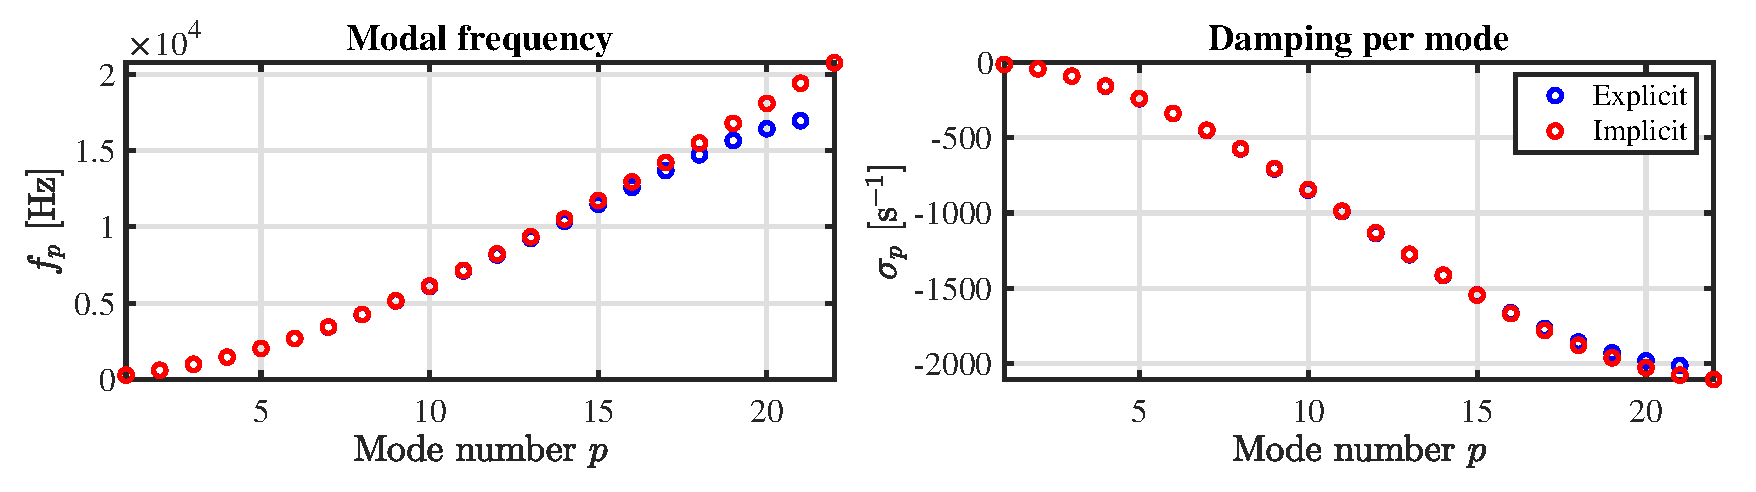
\includegraphics[width=\textwidth]{figures/resonators/implicitModes.eps}
    \caption{A comparison between the modal frequencies and damping per mode of the explicit (blue) and implicit (red) scheme. Here, $T = 1885$, $E = 2\cdot10^{14}$ and $\so = 1$ to highlight differences between the two schemes. One can observe that the modes of the implicit scheme follow the expected exponential pattern for the stiff string, where the explicit scheme shows numerically dispersive effects. Furthermore, due to the absence of $\so$ in the stability condition in Eq. \eqref{eq:implicitStability} and allows for one more grid point  \label{fig:implicitModes}}
\end{figure}

\subsection{Conclusion}
This section presented an implicit discretisation of the stiff string where the centred operator has been used to discretise the temporal derivative in the frequency-dependent damping term. By means of stability analysis and modal analysis some advantages that the implicit scheme has over its explicit counterpart (presented in Section \ref{sec:stiffStringDiscrete}) have been shown.

As these advantages only show for higher values of $\so$, much higher than the ones used in this project, it has been chosen to use the explicit scheme for all further implementation. The decrease in accuracy is negligible for lower values of $\so$ and the calculation of the scheme becomes orders of magnitude more computationally expensive if the implicit scheme is used. 